\chapter{Introductie}\label{introductie}

Vandaag de dag beschikken we over een enorme hoeveelheid aan digitale informatie. Ook wordt deze hoeveelheid aan informatie iedere dag groter en groter. 
In deze \textit{``Age of Big Data''} (\cite{lohr2012age}) bestaat de uitdaging erin om uit deze grote hoeveelheid data, door middel van analyse bepaalde inzichten te krijgen.
\\
Velen hebben dit probleem proberen aan te pakken, waarbij men zich vooral bezig hield met het brengen van structuur in deze grote dataset en zich voornamelijk concentreerde op onderwerp-gebaseerde classificatie. Echter met de opkomst van sociale media, blogs, reviewsites is er een groeiende interesse ontstaan voor gevoelsanalyse. Het onderzoek dat hiernaar gebeurd, heeft ook de nodige aandacht van bedrijven voor commerci\"ele toepassingen en ook zij spelen hierin een belangrijke rol.\\
%substukken
Als we over gevoelsanalyse spreken dan refereren we naar het verwerken van natuurlijke taal  om zo via tekstanalyse en computationele taalkunde subjectieve informatie uit te tekst te kunnen halen. Volgend voorbeeld illustreert een tweet waarop men bijvoorbeeld gevoelsanalyse kan uitvoeren.\\

\begin{figure}[h]%
    \centering
    \subfloat{{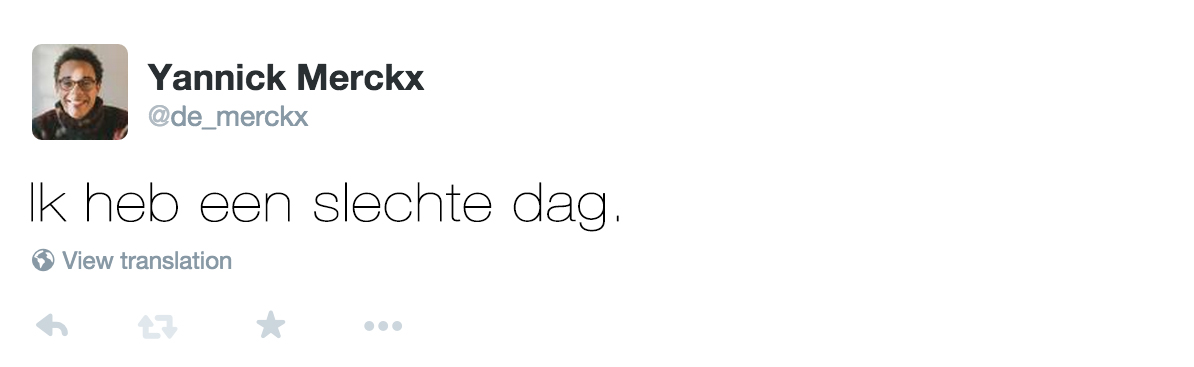
\includegraphics[width=10cm]{slechtedag} }}%
    \caption{een voorbeeldtweet voor gevoelsanalyse}%
\end{figure}

Verschillende technieken zijn hier mogelijk om de subjectiviteit of opinie uit deze tweet te bepalen. Men kan zich baseren op het woord \textit{slecht} en zo vaststellen dat de tweet een negatieve emotie uitdrukt. Maar men kan zich ook baseren op eerder vastgestelde tweets en op basis hiervan een beslissing nemen. Maar niet alles kan via gevoelsanalyse gedetecteerd worden bijvoorbeeld: stel dat dezelfde persoon juist de lotto had gewonnen en zich sarcastisch uitdrukte en juist een fantastische dag had. Het probleem rond sarcasme kan men vandaag de dag nog altijd niet oplossen met gevoelsanalyse(\cite{liebrecht2013perfect}).\\ 

Bijna al het onderzoek dat de afgelopen is jaren gebeurd met betrekking tot gevoelsanalyse werd uitgevoerd op Engelse teksten.Voornamelijk omdat het Engels een wereldtaal is en veel data beschikbaar is in het Engels. Daarentegen op het Nederlands is er weinig onderzoek uitgevoerd en is er veel minder data beschikbaar. Daarenboven bedrijven die dergelijk onderzoek uitvoeren op het Nederlands houden hun onderzoek (resultaten) ook vaak binnenshuis.
\\
Voor deze bachelorproef kijken we of de bevindingen over gevoelsanalyse op het Engels ook toepasbaar zijn op het Nederlands en/of er verschillen zijn tussen Nederlandse en Engelse gevoelsanalyse.
%workflow van wat je hebt gedaan
We zijn gestart met de voorbereiding van de bachelorproef in het 1ste semester met een verdieping in de literatuur over Engelse gevoelsanalyse. Verder maakte we ons vertrouwd met de programmeertaal Python, een van de programmeertalen bij uitstek die ons toelaat om experimentele analyses op te zetten.\\
Vervolgens zijn we op zoek gegaan naar onze data. Om de gevoelsanalyse te kunnen vergelijken, moet men zowel over een Engelse dataset als een Nederlandse dataset beschikken. Door het vele onderzoek naar Engelse gevoelsanalyse zijn er voldoende dataset beschikbaar op het web. Echter Nederlandse datasets, gelabeld volgens gevoel, zijn heel moeilijk te vinden en dwingt ons om de data manueel te scrapen. Voor het scrapen moeten we zoals eerder vermeld opletten voor sarcasme. Dit sluit scrapingsbronnen zoals Twitter en andere sociale media volledig uit. De volgende belangrijke volgende stap is het voorverwerken van de dataset bijvoorbeeld het verwijderen van stopwoorden. Om daarna het concept aan te leren aan zelflerende algoritmes. De zelflerende algoritmes met hun theoretische achtergrond worden besproken in hoofdstuk \ref{Lectuur}.\\

Vervolgens gaan we in hoofdstuk \ref{Experiment} over naar de experimentele analyse. Gebaseerd op gevonden resultaten in de literatuur voldoen reviewsites als \url{www.moviemeter.be} of \url{www.imdb.com} aan de criteria die we hadden vooropgesteld voor de experimentele analyse.  In sectie \ref{De Dataset} gaan we verder in op de scraping en verzamelde datasets. Initi\"eel om goed te doorgronden wat er juist gebeurd tijdens de voorverwerkingstechnieken, programmeren we deze technieken zelf voor de experimentele analyse. Later bij het dooranalyseren, optimaliseren we de code door gebruik te maken van de bibliotheek sklearn (\url{http://scikit-learn.org/}), die ons toelaat om sneller de analyses uit te voeren. Als eerste vergelijken de resultaten van de voorverwerkingstechnieken in combinatie met de leermethode op Nederlandse en Engelse filmrecensies.\\
Vervolgens concentreren we ons op de woordenschat en  onderzoeken we de classificatie op basis van een Engels en Nederlands geannoteerde woordenlijst van gevoelens.\\
Afhankelijk van het positieve karakter van de resultaten gaan we nog iets dieper in op Nederlandse gevoelsanalyse.\\
Na het experimentele analyse vormen we een conclusie of de gevonden technieken voor gevoelsanalyse op het Engels al dan niet toepasbaar zijn op het Nederlands. 